\newpage
\subsection{Caso d'uso UC3: Registrazione utente }
\label{UC3}
\begin{figure}[ht]
	\centering
	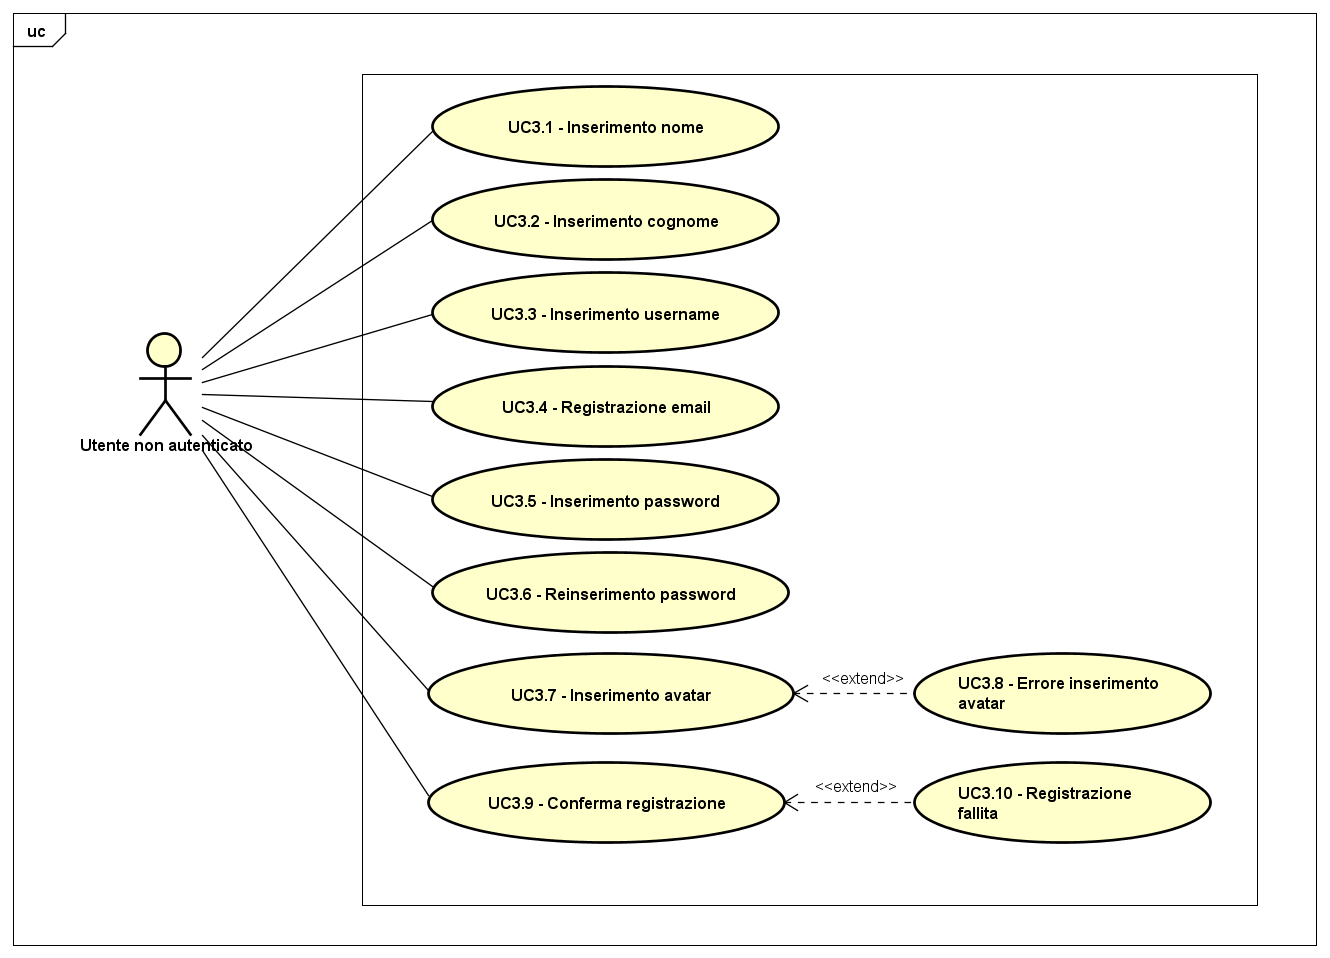
\includegraphics[scale=0.45]{UML/UC3.png}
	\caption{UC3: Registrazione utente}
\end{figure}

\begin{longtable}{ l | p{11cm}}
	\hline
	\rowcolor{Gray}
	 \multicolumn{2}{c}{UC3 - Registrazione utente} \\
	 \hline
	\textbf{Attori} & Utente non autenticato \\
	\textbf{Descrizione} & L'attore inserisce le sue informazioni personali per potersi registrare all'applicazione web, così da poter successivamente effettuare il login ed evolversi in un utente autenticato. \\
	\textbf{Pre-Condizioni} & L'attore ha scelto di registrarsi e l'applicazione web mostra la schermata di registrazione \\
	\textbf{Post-Condizioni} & L'attore si è registrato all'applicazione web \\
	\textbf{Scenario Principale} & 
	\begin{enumerate*}[label=(\arabic*.),itemjoin={\newline}]
		\item L'attore può inserire il proprio nome (UC3.1)
		\item L'attore può inserire il proprio cognome (UC3.2)
		\item L'attore può inserire lo username desiderato (UC3.3)
		\item L'attore può inserire la propria email (UC3.4) 
		\item L'attore può inserire la password desiderata (UC3.5)
		\item L'attore può reinserire la password desiderata per conferma (UC3.6)
		\item L'attore può inserire il proprio avatar (UC3.7)
		\item L'attore può confermare la registrazione (UC3.9)
	\end{enumerate*}\\
	\textbf{Scenari Alternativi} & 
	\begin{enumerate*}[label=(\arabic*.),itemjoin={\newline}]
		\item L'attore, durante il caricamento del file dell'avatar del nuovo utente, può visualizzare un messaggio di errore a riguardo, ed il caricamento del file non avviene (UC3.8)
		\item L'attore, alla conferma della registrazione, può visualizzare un messaggio d'errore che segnala i campi dati non validi (UC3.10)
	\end{enumerate*}\\
\end{longtable}

\subsubsection{Caso d'uso UC3.1: Inserimento nome}
\label{UC3_1}

\begin{longtable}{ l | p{11cm}}
	\hline
	\rowcolor{Gray}
	 \multicolumn{2}{c}{UC3.1 - Inserimento nome} \\
	 \hline
	\textbf{Attori} & Utente non autenticato \\
	\textbf{Descrizione} & L'attore inserisce il suo nome \\
	\textbf{Pre-Condizioni} & L'applicazione mostra il campo dati per l'inserimento del nome \\
	\textbf{Post-Condizioni} & L'attore ha inserito il proprio nome \\
	\textbf{Scenario Principale} & 
	\begin{enumerate*}[label=(\arabic*.),itemjoin={\newline}]
		\item L'attore può inserire il proprio nome
	\end{enumerate*}\\
\end{longtable}

\subsubsection{Caso d'uso UC3.2: Inserimento cognome}
\label{UC3_2}

\begin{longtable}{ l | p{11cm}}
	\hline
	\rowcolor{Gray}
	 \multicolumn{2}{c}{UC3.2 - Inserimento cognome} \\
	 \hline
	\textbf{Attori} & Utente non autenticato \\
	\textbf{Descrizione} & L'attore inserisce il suo cognome \\
	\textbf{Pre-Condizioni} & L'applicazione mostra il campo dati per l'inserimento del cognome \\
	\textbf{Post-Condizioni} & L'attore ha inserito il proprio cognome \\
	\textbf{Scenario Principale} & 
	\begin{enumerate*}[label=(\arabic*.),itemjoin={\newline}]
		\item L'attore può inserire il proprio cognome
	\end{enumerate*}\\
\end{longtable}

\subsubsection{Caso d'uso UC3.3: Inserimento username}
\label{UC3_3}

\begin{longtable}{ l | p{11cm}}
	\hline
	\rowcolor{Gray}
	 \multicolumn{2}{c}{UC3.3: Inserimento username} \\
	 \hline
	\textbf{Attori} & Utente non autenticato \\
	\textbf{Descrizione} & L'attore inserisce lo username desiderato \\
	\textbf{Pre-Condizioni} & L'applicazione mostra il campo dati per l'inserimento dello username \\
	\textbf{Post-Condizioni} & L'attore ha inserito lo username desiderato \\
	\textbf{Scenario Principale} & 
	\begin{enumerate*}[label=(\arabic*.),itemjoin={\newline}]
		\item L'attore può inserire lo username desiderato
	\end{enumerate*}\\
\end{longtable}

\subsubsection{Caso d'uso UC3.4: Registrazione email}
\label{UC3_4}

\begin{longtable}{ l | p{11cm}}
	\hline
	\rowcolor{Gray}
	 \multicolumn{2}{c}{UC3.4 - Registrazione email} \\
	 \hline
	\textbf{Attori} & Utente non autenticato \\
	\textbf{Descrizione} & L'attore registra la propria email \\
	\textbf{Pre-Condizioni} & L'applicazione mostra il campo dati per la registrazione dell'email \\
	\textbf{Post-Condizioni} & L'attore ha registrato la propria email \\
	\textbf{Scenario Principale} & 
	\begin{enumerate*}[label=(\arabic*.),itemjoin={\newline}]
		\item L'attore può registrare la propria email
	\end{enumerate*}
\end{longtable}

\subsubsection{Caso d'uso UC3.5: Inserimento password}
\label{UC3_5}

\begin{longtable}{ l | p{11cm}}
	\hline
	\rowcolor{Gray}
	 \multicolumn{2}{c}{UC3.5 - Inserimento password} \\
	 \hline
	\textbf{Attori} & Utente non autenticato \\
	\textbf{Descrizione} & L'attore inserisce la password desiderata  \\
	\textbf{Pre-Condizioni} & L'applicazione mostra il campo dati per l'inserimento della password \\
	\textbf{Post-Condizioni} & L'attore ha inserito la password desiderata \\
	\textbf{Scenario Principale} & 
	\begin{enumerate*}[label=(\arabic*.),itemjoin={\newline}]
		\item L'attore può inserire la password desiderata
	\end{enumerate*}\\
\end{longtable}

\subsubsection{Caso d'uso UC3.6: Reinserimento password}
\label{UC3_6}

\begin{longtable}{ l | p{11cm}}
	\hline
	\rowcolor{Gray}
	 \multicolumn{2}{c}{UC3.6 - Reinserimento password} \\
	 \hline
	\textbf{Attori} & Utente non autenticato \\
	\textbf{Descrizione} & L'attore reinserisce la password desiderata  \\
	\textbf{Pre-Condizioni} & L'applicazione mostra il campo dati per il reinserimento della password \\
	\textbf{Post-Condizioni} & L'attore ha reinserito la password desiderata \\
	\textbf{Scenario Principale} & 
	\begin{enumerate*}[label=(\arabic*.),itemjoin={\newline}]
		\item L'attore può reinserire la password desiderata
	\end{enumerate*}\\
\end{longtable}

\subsubsection{Caso d'uso UC3.7: Inserimento avatar}
\label{UC3_7}

\begin{minipage}{\linewidth}
	\begin{tabular}{ l | p{11cm}}
		\hline
		\rowcolor{Gray}
		\multicolumn{2}{c}{UC3.7 - Inserimento avatar} \\
		\hline
		\textbf{Attori} & Utente non autenticato \\
		\textbf{Descrizione} & L'attore carica su API Market un file contenente l'avatar per il nuovo utente \\
		\textbf{Pre-Condizioni} & L'attore si trova nella schermata relativa alla registrazione di un nuovo utente \\
		\textbf{Post-Condizioni} & L'attore ha caricato su API Market un file contenente l'avatar per il nuovo utente \\
		\textbf{Scenario Principale} & 
		\begin{enumerate*}[label=(\arabic*.),itemjoin={\newline}]
			\item L'attore può caricare su API Market un file contenente l'avatar per il nuovo utente
		\end{enumerate*}\\
		\textbf{Scenari Alternativi} & 
		\begin{enumerate*}[label=(\arabic*.),itemjoin={\newline}]
		\item L'attore può visualizzare un messaggio di errore (E.g: formato errato) ed il caricamento del file non avviene (UC3.8)
		\end{enumerate*}\\
	\end{tabular}
\end{minipage}

\subsubsection{Caso d'uso UC3.8: Errore inserimento avatar}
\label{UC3_8}

\begin{minipage}{\linewidth}
	\begin{tabular}{ l | p{11cm}}
		\hline
		\rowcolor{Gray}
		\multicolumn{2}{c}{UC3.8 - Errore inserimento avatar} \\
		\hline
		\textbf{Attori} & Utente non autenticato \\
		\textbf{Descrizione} & L'attore visualizza un messaggio di errore e l'inserimento dell'avatar per il nuovo utente non avviene \\
		\textbf{Pre-Condizioni} & L'attore ha cercato di caricare su API Market un file contenente l'avatar per il nuovo utente ma si è verificato un errore \\
		\textbf{Post-Condizioni} & L'attore ha visualizzato un messaggio di errore \\
		\textbf{Scenario Principale} & 
		\begin{enumerate*}[label=(\arabic*.),itemjoin={\newline}]
			\item L'attore può visualizzare un messaggio di errore (E.g: formato non valido)
		\end{enumerate*}\\
	\end{tabular}
\end{minipage}

\subsubsection{Caso d'uso UC3.9: Conferma registrazione}
\label{UC3_9}

\begin{longtable}{ l | p{11cm}}
	\hline
	\rowcolor{Gray}
	 \multicolumn{2}{c}{UC3.9 - Conferma registrazione} \\
	 \hline
	\textbf{Attori} & Utente non autenticato \\
	\textbf{Descrizione} & L'attore conferma i dati inseriti per la registrazione \\
	\textbf{Pre-Condizioni} & L'applicazione mostra il pulsante per la conferma della registrazione (con le informazioni inserite nei campi dati) \\
	\textbf{Post-Condizioni} & L'attore ha confermato la registrazione, visualizzando il messaggio di successo, ed è stato reindirizzato alla pagina principale come utente non autenticato (UC1) \\
	\textbf{Scenario Principale} & 
	\begin{enumerate*}[label=(\arabic*.),itemjoin={\newline}]
		\item L'attore può confermare la registrazione, visualizzando il messaggio di successo, e venendo reindirizzato alla pagina principale come utente non autenticato (UC1)
	\end{enumerate*}\\
\end{longtable}

\subsubsection{Caso d'uso UC3.10: Registrazione fallita}
\label{UC3_10}

\begin{minipage}{\linewidth}
	\begin{longtable}{ l | p{11cm}}
		\hline
		\rowcolor{Gray}
	 	\multicolumn{2}{c}{UC3.10 - Registrazione fallita} \\
	 	\hline
		\textbf{Attori} & Utente non autenticato \\
		\textbf{Descrizione} & L'attore fallisce la registrazione  \\
		\textbf{Pre-Condizioni} & L'attore ha confermato i dati inseriti \\
		\textbf{Post-Condizioni} & L'attore ha visualizzato un messaggio d'errore che segnala i campi dati non validi \\
		\textbf{Scenario Principale} & 
		\begin{enumerate*}[label=(\arabic*.),itemjoin={\newline}]
			\item L'attore può visualizzare un messaggio d'errore che segnala i campi dati non validi (E.g: Campi dati vuoti, caratteri speciali, username o email già presenti) 
		\end{enumerate*}\\
	\end{longtable}
\end{minipage}